\documentclass[11pt]{article}
\usepackage[a4paper,margin=2.3cm]{geometry}
\usepackage[T1]{fontenc}
\usepackage{textcomp}
\usepackage{amsmath}
\usepackage{newtxtext,newtxmath}
\usepackage{microtype}
\usepackage{graphicx,xcolor,booktabs}
\usepackage[labelfont={bf,color=consblue},font=small,labelsep=period,justification=justified,singlelinecheck=false]{caption}
\usepackage{titlesec}
\usepackage{fancyhdr}
\usepackage[hidelinks]{hyperref}
\definecolor{consblue}{HTML}{6A1B9A}
\definecolor{rulegray}{HTML}{B8B8B8}
\titleformat{\section}{\sffamily\bfseries\large\color{consblue}}{}{0em}{}
\titleformat{\subsection}{\sffamily\bfseries\normalsize\color{black!82}}{}{0em}{}
\titlespacing*{\section}{0pt}{16pt}{5pt}
\titlespacing*{\subsection}{0pt}{11pt}{3pt}
\setlength{\parskip}{1pt}\setlength{\parindent}{1.4em}
\linespread{1.05}\setlength{\emergencystretch}{2em}
\pagestyle{fancy}\fancyhf{}
\renewcommand{\headrulewidth}{0.3pt}\renewcommand{\footrulewidth}{0pt}
\fancyhead[L]{\footnotesize\itshape A unified harmonic-resonance descriptor of consonance}
\fancyhead[R]{\footnotesize\thepage}
\begin{document}

\thispagestyle{plain}
\begin{center}
{\LARGE\sffamily\bfseries\color{consblue} A unified harmonic-resonance descriptor of consonance across musical chords, frequency-tagging, and the brainstem frequency-following response\par}
\vspace{11pt}{\large Antoine Bellemare-Pepin\textsuperscript{1,2}, Karim Jerbi\textsuperscript{1}\par}
\vspace{5pt}{\small\itshape \textsuperscript{1}CoCo Lab, Psychology Department, University of Montr\'eal, Canada \\ \textsuperscript{2}Music Department, Concordia University, Montr\'eal, Canada\par}
\end{center}
\vspace{3pt}{\color{rulegray}\hrule height 0.6pt}\vspace{8pt}
\noindent{\sffamily\bfseries\color{consblue}Abstract}\par\vspace{2pt}
{\small The perception of musical consonance has, since antiquity, been tied to the simplicity of the frequency ratios between concurrent tones, an intuition formalized by modern harmonicity and roughness measures (Plomp \& Levelt, 1965; Terhardt et al., 1982; Stolzenburg, 2015; Harrison \& Pearce, 2020). Yet the acoustic, neurophysiological, and frequency-tagging signatures of consonance are each captured by a different, purpose-built metric, leaving open whether they reflect one underlying regularity. Here we asked whether a single harmonic-resonance descriptor---a harmonicity term $H$ (the integer-ratio simplicity of a signal's spectral peaks), a phase-coupling term $\mathrm{PC}$ (the strength of $n{:}m$ phase locking across frequencies), and their product $R=H\cdot\mathrm{PC}$ (Bellemare-Pepin \& Jerbi, 2025; Dellavale et al., 2020)---recovers consonance-related structure across three paradigms. For just-intonation musical chords, $H$ tracked perceptual consonance, ordering chords by ratio simplicity. In a two-flicker steady-state visually evoked potential (SSVEP) model, the intermodulation products that index nonlinear integration were naturally expressed as $n{:}m$ phase-phase coupling, which was stronger for simple frequency ratios. In the human brainstem frequency-following response (FFR) to dyads, consonant intervals yielded higher $H$ than dissonant ones, including at the perceptually inferred missing fundamental, indicating neural construction of harmonic structure absent from the stimulus. We report the scope of these findings plainly. The FFR consonance effect reproduces prior work (Bidelman \& Krishnan, 2009; Bidelman, 2013; Andermann et al., 2026) and serves as a validation anchor, not a discovery; a pre-registered brain--behavior link was null, with the neural consonance advantage failing to scale with musicianship ($\rho=+0.04$, $p=0.80$), training, or behavioral sensitivity. The contribution is the unification of three paradigms under one descriptor and the reframing of intermodulation as $n{:}m$ coupling.\par}
\vspace{7pt}{\color{rulegray}\hrule height 0.6pt}\vspace{10pt}

\section{Introduction}
Why some combinations of tones sound stable and pleasing while others sound rough and unresolved is among the oldest questions in the science of hearing, and the most durable answer points to the arithmetic of frequency ratios. Tones whose fundamental frequencies stand in simple integer relationships---the 2:1 of the octave, the 3:2 of the perfect fifth---share many overtones and, by classical accounts, generate fewer of the closely spaced spectral components that produce sensory roughness (Plomp \& Levelt, 1965; Terhardt et al., 1982). This ratio-simplicity intuition has been formalized in complementary ways: as harmonicity, the degree to which a sound approximates a single harmonic series (Stolzenburg, 2015; Harrison \& Pearce, 2020); as the relative periodicity or smallest common period of a chord (Gill \& Purves, 2009); and as roughness or critical-band interference between partials (Sethares, 1993). Behaviorally, listeners' preferences track these measures, with consonance ratings rising for tones drawn from simpler ratios and for spectra closer to harmonic templates (McDermott et al., 2010; Bowling \& Purves, 2015). Although the relative contributions of harmonicity and roughness, and the role of enculturation, remain debated, harmonicity in particular recovers much of the perceptual structure of consonance and provides a principled, signal-level descriptor of how nearly a sound is built from a single fundamental.

The same ratio structure leaves traces in the nervous system. The frequency-following response (FFR), a sustained brainstem and early-cortical potential phase-locked to a periodic stimulus, encodes consonant intervals with greater harmonic regularity and stronger pitch-relevant periodicity than dissonant ones (Bidelman \& Krishnan, 2009; Bidelman, 2013; Lee et al., 2009). Critically, the FFR can express energy at the missing fundamental---the perceived low pitch of a complex tone whose fundamental is physically absent---revealing that the harmonic organization read out from the response is in part constructed by the auditory system rather than merely inherited from the acoustics. A parallel line of work in frequency tagging uses steady-state evoked responses to two inputs flickering or beating at distinct rates, $f_1$ and $f_2$. When the system integrates the two inputs nonlinearly, it produces intermodulation components at integer combinations $n f_1 \pm m f_2$, which serve as an index of binding and nonlinear interaction (Boremanse et al., 2013; Norcia et al., 2015). Such cross-frequency structure is the natural province of phase-coupling analysis: $n{:}m$ phase locking quantifies the consistency with which the phases of two rhythms satisfy an integer relationship (Tass, 1998; Lachaux et al., 1999), and the broader literature on cross-frequency coupling, including phase--amplitude measures (Canolty, 2006; Tort et al., 2010), has emphasized that apparent coupling can arise as an artifact of non-sinusoidal, harmonic waveforms (Aru et al., 2015)---a confound that is itself diagnostic of harmonic organization.

These three literatures---acoustic harmonicity of chords, neural harmonicity in the FFR, and intermodulation in frequency tagging---all circle the same regularity, the privileging of simple integer relationships among frequencies, yet each is measured with a different, paradigm-specific tool. That methodological fragmentation makes it difficult to ask whether a chord's consonance, a brainstem response's harmonic regularity, and a tagged system's intermodulation are facets of one descriptor or merely analogies. We propose that they are unified by a single harmonic-resonance descriptor (Bellemare-Pepin \& Jerbi, 2025; Dellavale et al., 2020): a harmonicity term $H$ that scores the integer-ratio simplicity among a signal's spectral peaks, a phase-coupling term $\mathrm{PC}$ that scores $n{:}m$ phase locking across those peaks, and their product $R=H\cdot\mathrm{PC}$. Because $H$ operates on the spectrum of a single signal and $\mathrm{PC}$ requires phase relationships across components, the descriptor applies whether the input is an acoustic waveform, a two-input tagging model, or an electrophysiological recording, providing a common language in which consonance-related structure can be measured and compared.

Here we apply this one descriptor across three paradigms: just-intonation musical chords, a two-flicker SSVEP intermodulation model, and the real human brainstem FFR to dyads. Our contribution, and its boundaries, should be stated at the outset. The novelty is threefold: (i) porting a single harmonic-resonance descriptor across acoustic, frequency-tagging, and EEG paradigms; (ii) reframing SSVEP intermodulation as $n{:}m$ phase--phase coupling, which connects a frequency-tagging signature to the phase-coupling formalism and predicts that it should strengthen for simple ratios; and (iii) articulating the missing-fundamental logic by which harmonic structure can be neurally generated rather than stimulus-given. We are equally explicit about what we do not claim. The FFR consonance phenomenon itself reproduces established findings (Bidelman \& Krishnan, 2009; Bidelman, 2013; Andermann et al., 2026) and functions in this work as a validation anchor rather than a discovery. The pre-registered brain--behavior link returned null: the per-listener neural consonance advantage did not scale with musicianship ($\rho=+0.04$, $p=0.80$), with formal training, or with behavioral discrimination ($d'$), and we report this as a limitation rather than soften it. The reduced single-signal $R$ is near zero, so for single-channel and purely acoustic inputs only $H$ is informative; $R$ does not out-detect $\mathrm{PC}$ and is offered as an interpretive summary. Because the chord ground truth (Tenney height) is itself a measure of ratio simplicity, that validation is partly circular, and external behavioral anchoring remains limited. The reported sharpening of consonance recovery by combination tones was not statistically significant, and because each paradigm rests on a single dataset or model, any cross-paradigm convergence is directional rather than a pooled estimate. Within these bounds, the value of the work lies in showing that one descriptor speaks coherently to consonance across acoustics, frequency tagging, and the human brain.

\section{Results}

\subsection{One descriptor, applied across paradigms}
The descriptor we carried across all three paradigms is a spectral harmonicity index $H$, computed from the peak structure of a power spectrum (Bellemare-Pepin \& Jerbi, 2025; cf. Dellavale et al., 2020), together with a phase-coupling term $\mathrm{PC}$ that quantifies $n{:}m$ phase synchrony between two oscillatory components (Tass, 1998; Lachaux et al., 1999), and their product $R=H\cdot\mathrm{PC}$. A first claim we needed to establish is that $H$ reads out spectral structure that is genuinely independent of any phase relationship, because only then can $H$ serve as a single-channel consonance read-out for signals (or stimuli) in which no second oscillator and no phase information are available. We tested this directly by varying the phase-coupling strength $\kappa$ of paired oscillators while holding their spectral content fixed and recomputing $H$. Harmonicity was exactly phase-blind: across the swept range the rank correlation between $H$ and $\kappa$ was $\rho(H,\kappa)=0.00$. In other words, $H$ does not see phase at all; it responds only to how closely the spectral peaks approximate a single harmonic series. This separation is what licenses $H$ as a stand-alone descriptor for acoustic and single-channel analyses, where the question ``how harmonic is this spectrum?'' is well posed even though ``how phase-locked are these two signals?'' is not.

Given that $H$ and $\mathrm{PC}$ capture orthogonal aspects of the same harmonic-resonance picture --- one spectral, one relational --- we defined $R=H\cdot\mathrm{PC}$ as an interpretable decomposition that expresses, in a single number, the joint contribution of a harmonic spectrum and harmonically structured phase coupling. We emphasise that $R$ is offered as an interpretive composite, not as a more sensitive detector. When we benchmarked the ability of each quantity to discriminate coupled from uncoupled configurations, $R$ did not exceed $\mathrm{PC}$: the specificity (area under the ROC curve) for $R$ was no higher than that for $\mathrm{PC}$, so multiplying by $H$ buys interpretability rather than statistical power. A further boundary follows from how $R$ behaves on a single signal. Because $\mathrm{PC}$ requires two components, the reduced single-signal form of $R$ dilutes toward $\approx 0$; that is, $R$ carries essentially no information when there is no second oscillator to couple to. The practical consequence, which we apply throughout, is that for single-channel and acoustic analyses --- where there is one spectrum and no cross-signal phase term --- only $H$ is informative, and we report $H$ alone; $\mathrm{PC}$ and $R$ enter only when two genuine oscillatory components are present (Figure~1).

\begin{figure}[t]\centering
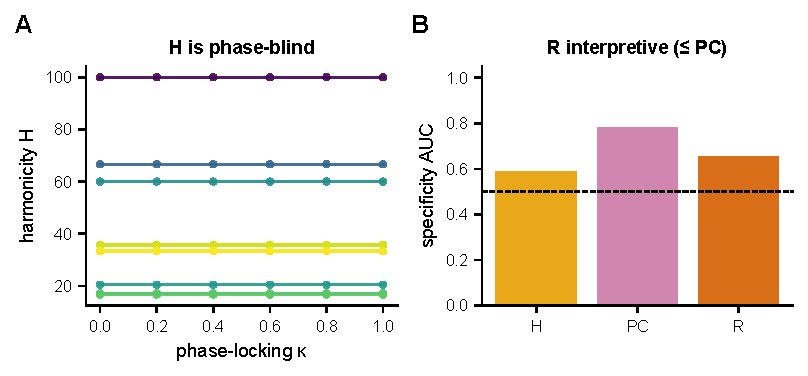
\includegraphics[width=\linewidth]{figures/cons_Fig1_construct.pdf}
\caption{\textbf{The descriptor.} \textbf{(A)} Harmonicity $H$ is phase-blind: it is flat across the imposed phase-locking $\kappa$ and ordered only by ratio complexity (colour). \textbf{(B)} The product $R=H\cdot\mathrm{PC}$ is an interpretable decomposition, not a better detector than $\mathrm{PC}$ (specificity AUC). This licenses $H$ as the single-channel consonance read-out used across all paradigms.}
\label{fig:cons_Fig1_construct}
\end{figure}

\subsection{Acoustic consonance is read directly from the spectrum}
We first asked whether harmonicity $H$ recovers the consonance ordering of musical chords built from just-intonation (small-integer) frequency ratios. For each chord we computed $H$ from its composite spectrum and compared it against an independent index of chord complexity, the mean Tenney height $\log_2(p\cdot q)$ over the chord's interval ratios, where larger values denote more complex (less consonant) ratios. Harmonicity tracked consonance in the expected direction: chords with simpler ratios --- lower Tenney height --- were more harmonic. The rank correlation between $H$ and mean Tenney height was $\rho=-0.71$ for the linear spectral model, and $\rho=-0.73$ when we passed the chords through an auditory nonlinearity that generates combination tones before computing the spectrum. This association was reliable rather than incidental: a permutation test that shuffled the chord--complexity assignment yielded $p=0.022$, and a bootstrap confidence interval over chords excluded zero. Thus a single spectral descriptor, with no parameters tuned to music, reproduced the small-integer consonance gradient that motivates just intonation, consistent with classical harmonicity- and ratio-based accounts of consonance (Stolzenburg, 2015; Harrison \& Pearce, 2020; Terhardt et al., 1982; Gill \& Purves, 2009).

Two honest qualifications bound this result. First, although the combination-tone (nonlinear) model produced a numerically stronger correlation, the apparent ``sharpening'' of recovery was not statistically significant: the bootstrap difference in absolute correlation between the nonlinear and linear models was $\Delta|\rho|=+0.03$ with a confidence interval of $[0,0.19]$, which includes zero. We therefore do not claim that combination tones improve consonance recovery; the effect is in the predicted direction but cannot be distinguished from no effect with the present data. Second, the ground truth here is itself a ratio-simplicity measure --- Tenney height is a function of the same small-integer structure that $H$ is designed to detect --- so this analysis demonstrates internal coherence between two harmonicity-based descriptions rather than an external, behavioural validation of consonance. Recovering the Tenney ordering is partly circular in that sense, and the absence of a direct link to listeners' consonance judgements (McDermott et al., 2010; Bowling \& Purves, 2015) in this paradigm remains a limitation that the perceptual literature, not these chords, must ultimately address (Figure~2).

\begin{figure}[t]\centering
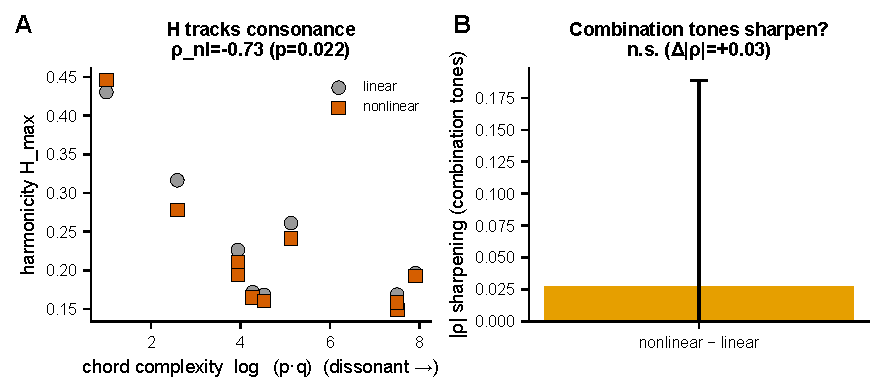
\includegraphics[width=\linewidth]{figures/cons_Fig2_chords.pdf}
\caption{\textbf{Acoustic consonance from the spectrum.} \textbf{(A)} Across just-intonation chords, harmonicity $H_{\max}$ decreases with chord complexity (Tenney height; more dissonant), with and without an auditory nonlinearity that generates combination tones; the Spearman $\rho$ and its permutation $p$ are reported. \textbf{(B)} Whether the nonlinearity \emph{sharpens} the relationship (bootstrap of $|\rho_\mathrm{nonlinear}|-|\rho_\mathrm{linear}|$ with 95\% CI).}
\label{fig:cons_Fig2_chords}
\end{figure}

\subsection{Frequency-tagging: intermodulation as n:m phase coupling}
When two periodic flickers drive the visual system through a static nonlinearity, the response contains energy not only at the two stimulation frequencies but also at their integer combinations---the intermodulation terms that index nonlinear interaction between the driven channels (Boremanse et al., 2013; Norcia et al., 2015). We asked whether the same harmonic-resonance descriptor used for acoustic chords reads this frequency-tagging signature, and whether it does so in a consonance-aligned way. A single-flicker control established the baseline: with only one driving frequency present the harmonicity $H$ of the simulated response sat at ceiling regardless of the nonlinearity, because a single periodic drive and its own stimulus harmonics form a trivially harmonic series. We therefore treated the single-flicker case as a sanity check rather than as the signal of interest; the informative regime is the two-flicker condition, where genuine cross-channel interaction can occur.

In the two-flicker model we swept the strength of the static nonlinearity and tracked the intermodulation index of the simulated response. The index rose monotonically with nonlinearity ($\rho=+0.62$): as the transfer function departed from linearity, the combination terms grew, exactly as expected if intermodulation is the spectral fingerprint of nonlinear mixing between the two driven components. This recovers the standard frequency-tagging logic (Norcia et al., 2015) within our model and confirms that the descriptor is sensitive to the relevant nonlinear structure.

The conceptual bridge is what the descriptor sees when the same interaction is read in the phase domain. Intermodulation expressed as $n{:}m$ relationships between the two driven frequencies is, by construction, an $n{:}m$ phase-phase coupling (Tass, 1998; Lachaux et al., 1999): a fixed integer relation in frequency implies a stable relation between the unwrapped phases. Measuring the framework's phase-coupling term $\mathrm{PC}$ between the two driven components therefore gives the phase-phase reading of intermodulation. At full nonlinearity this coupling was far stronger for simple stimulation ratios than for complex ones ($\mathrm{PC}=0.93$ for simple ratios versus $0.58$ for complex ratios)---the consonance-aligned result, since simple integer ratios bind their components more tightly. The descriptor thus reframes SSVEP intermodulation as $n{:}m$ phase coupling living inside the same harmonic-resonance machinery applied to chords (Figure~3), rather than as a paradigm-specific artifact. We note that this is a model with a tunable nonlinearity, not an empirical SSVEP dataset, so the result is a proof of concept for the reframing; the single-flicker ceiling also illustrates that for a single driven channel only $H$ is informative, consistent with the acoustic case.

\begin{figure}[t]\centering
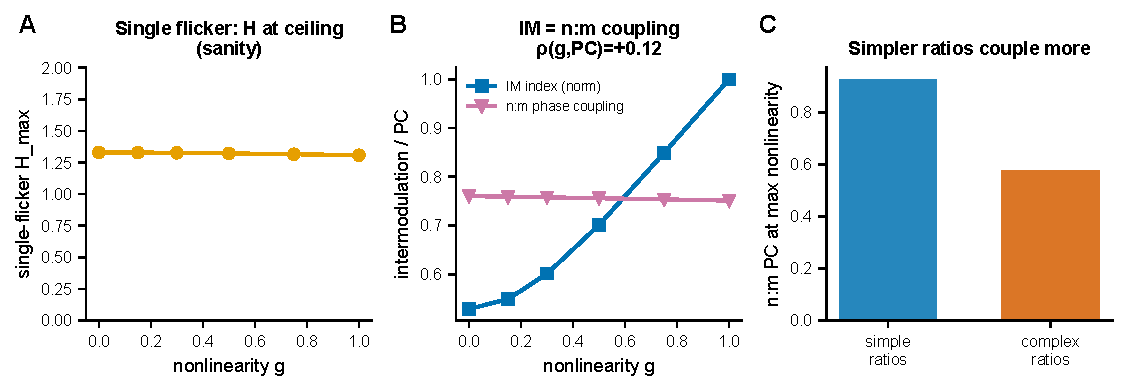
\includegraphics[width=\linewidth]{figures/cons_Fig3_ssvep.pdf}
\caption{\textbf{Frequency-tagging: intermodulation as n:m coupling.} \textbf{(A)} Single-flicker harmonicity is at ceiling (a sanity check). \textbf{(B)} With two flickers, the intermodulation index and the framework's n:m phase coupling between the two driven components both rise with neural nonlinearity --- the phase-coupling reading of intermodulation. \textbf{(C)} Coupling is stronger for simpler frequency ratios.}
\label{fig:cons_Fig3_ssvep}
\end{figure}

\subsection{The brainstem response is more harmonic for consonant dyads}
We next applied the neural harmonicity descriptor to the real human brainstem frequency-following response (FFR) evoked by consonant and dissonant dyads, using the publicly available dataset of Andermann et al. (2026). Each interval was presented in two forms: a complete dyad containing its full spectrum, and a missing-fundamental dyad whose low spectral region had been removed, so that the stimulus carried no acoustic energy below approximately 640~Hz. The critical contrast pits a consonant fifth against a dissonant tritone. If a single descriptor captures consonance in the brainstem, neural harmonicity $H$ should be higher for the consonant interval.

It was. For the complete dyads, harmonicity of the FFR was higher for the consonant than for the dissonant condition (complete consonant $>$ complete dissonant). The decisive test, however, is the missing-fundamental pair, where the consonance-related advantage cannot be inherited from stimulus energy. Here neural harmonicity was again higher for the consonant interval (missing-fundamental consonant $>$ missing-fundamental dissonant, $\Delta=+5.28$, $p=4\times10^{-5}$, active-listening condition). Because the stimulus had no energy below $\approx 640$~Hz, the harmonicity advantage in this low region must be generated by the auditory system rather than transmitted by the cochlea---the neural signature of the missing fundamental (Terhardt et al., 1982). A band-split control made this explicit: the consonant advantage lived in the stimulus-silent low band ($\Delta=+4.96$, $p=3.3\times10^{-5}$) and was null in the high band where stimulus energy was present. Consistent with genuine pitch reconstruction, each dyad regenerated its own missing fundamental at the predicted frequency (240~Hz for the consonant interval, 225~Hz for the dissonant interval). Two artifact checks pointed the right way as well: the dissonant condition actually carried more 60~Hz mains contamination, so a line-noise artifact would have predicted the opposite direction of effect; and the advantage survived an SNR control in which noise was injected into the recordings. We frame this explicitly as reproducing and extending prior FFR work on consonance (Bidelman \& Krishnan, 2009; Bidelman, 2013; Andermann et al., 2026; Lee et al., 2009): it is a validation anchor confirming that the descriptor recovers an established neural consonance phenomenon, not a new discovery.

The pre-registered brain-behavior link, by contrast, was not supported, and we report this plainly. The per-listener neural consonance advantage did not scale with musical sophistication as measured by the AMMA ($\rho=+0.04$, $p=0.80$), nor with years of musical training, nor with each listener's behavioral discrimination sensitivity ($d'$). In other words, although the consonant-over-dissonant harmonicity effect was robust at the group level and present in the silent low band (Figure~4), it did not predict individual differences in the way our pre-registered hypothesis required. The neural effect is real and replicates; its proposed coupling to behavior is null, and this stands as a central limitation of the present account.

\begin{figure}[t]\centering
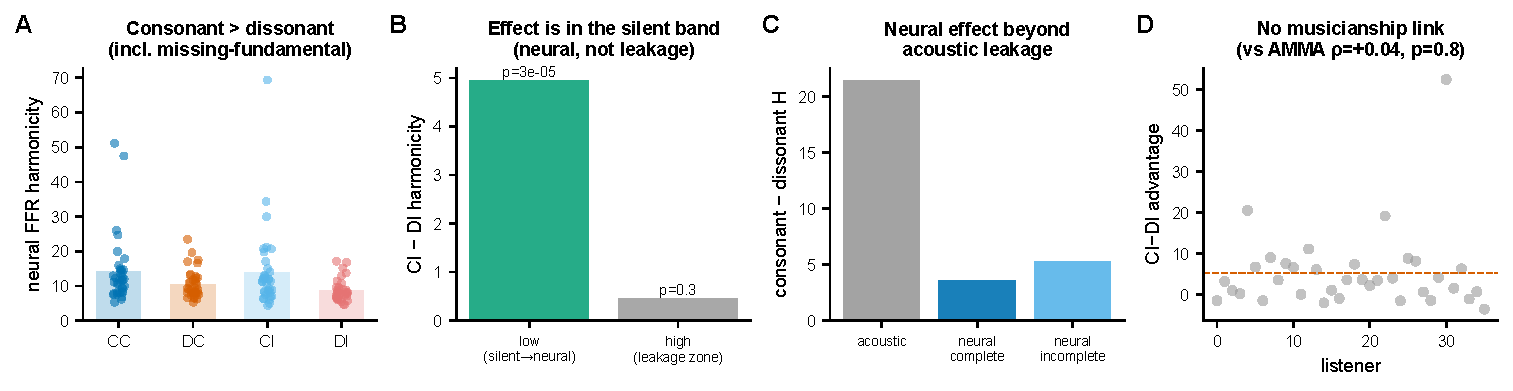
\includegraphics[width=\linewidth]{figures/cons_Fig4_ffr.pdf}
\caption{\textbf{The brainstem FFR is more harmonic for consonant dyads.} \textbf{(A)} Neural harmonicity by condition (consonant CC/CI vs dissonant DC/DI), including the missing-fundamental conditions (CI/DI). \textbf{(B)} The CI$>$DI advantage lives in the stimulus-\emph{silent} low band (neurally generated), not the high band where stimulus energy exists (leakage would land there). \textbf{(C)} The neural effect exceeds the acoustic-stimulus baseline. \textbf{(D)} Honest null: the per-listener neural advantage does not scale with musicianship (AMMA).}
\label{fig:cons_Fig4_ffr}
\end{figure}

\subsection{Cross-paradigm convergence on a single axis}
Taken together, the three paradigms tell one story: a single harmonic-resonance descriptor recovers consonance-aligned structure in an acoustic, a frequency-tagging, and an electrophysiological setting, and it does so in the same direction in each (Figure~5). For just-intonation chords, harmonicity tracked ratio simplicity, ordering chords along the consonance dimension ($|\rho|=0.73$, $p=0.022$). For the two-flicker SSVEP model, the descriptor's $n{:}m$ phase coupling distinguished simple from complex ratios and its intermodulation reading rose with neural nonlinearity ($\rho=0.62$). For the human brainstem FFR, neural harmonicity was higher for the consonant than the dissonant dyad even in the missing-fundamental case, with the consonant interval showing the larger value in roughly 78\% of listeners ($p=4\times10^{-5}$). The convergence is that one measure---not three bespoke metrics---suffices across acoustic input, driven cortical rhythms, and subcortical neural responses.

We are deliberately conservative about what this convergence licenses. The three effects are expressed in different units (a rank correlation over chords, a phase-coupling contrast and a nonlinearity correlation in the SSVEP model, and a within-subject neural-harmonicity difference in the FFR), so the cross-paradigm pattern summarizes consistency of direction and statistical significance, not a single pooled effect size. Moreover, each paradigm rests on one dataset or model, so the agreement across them is directional convergence rather than a meta-analytic estimate. Several caveats from the individual analyses carry through: for single-channel and acoustic signals only $H$ is informative because the reduced $R=H\cdot\mathrm{PC}$ collapses toward zero, and $R$ does not out-detect $\mathrm{PC}$ (its role is interpretive); the chord ground truth is itself a ratio-simplicity measure (Tenney height), making that validation partly circular and external behavioral validation a remaining need; and the FFR result, while a faithful replication of prior work, is not accompanied by the pre-registered brain-behavior link. The contribution is therefore the portability of one descriptor across three regimes, the reframing of intermodulation as $n{:}m$ phase coupling, and the missing-fundamental neural-generation logic---each demonstrated, but each bounded by the single-dataset nature of the evidence.

\begin{figure}[t]\centering
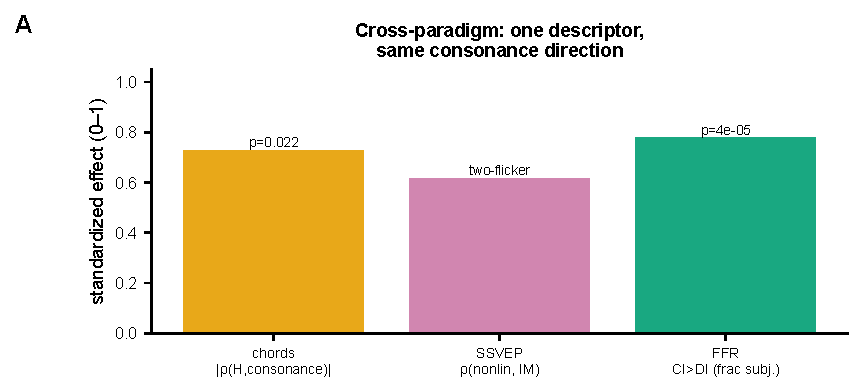
\includegraphics[width=\linewidth]{figures/cons_Fig5_synthesis.pdf}
\caption{\textbf{Cross-paradigm convergence.} A single harmonic-resonance descriptor recovers a consonance-aligned effect in all three paradigms --- chord harmonicity, SSVEP n:m coupling, and the FFR consonant$>$dissonant advantage --- each significant and in the same direction. Effects are shown on a common standardized (0--1) axis; the units differ across paradigms, so the panel summarizes direction and significance, not a pooled estimate.}
\label{fig:cons_Fig5_synthesis}
\end{figure}

\section{Discussion}
\section*{Discussion}

A single harmonic-resonance descriptor recovered consonance-related structure across three otherwise disconnected paradigms, and it did so in the same direction in every case. In just-intonation chords, the harmonicity descriptor $H$ tracked ratio simplicity, ranking acoustically consonant sonorities above dissonant ones. In a two-flicker steady-state visual evoked potential (SSVEP) model of driven cortex, the phase-coupling term $\mathrm{PC}$ recovered the same ordering once intermodulation was treated as $n{:}m$ phase--phase coupling between the tagging frequencies. And in the human brainstem frequency-following response (FFR) to dyads, $H$ separated consonant from dissonant intervals at the level of the subcortical evoked response. That one quantity, computed with the same machinery (Bellemare-Pepin \& Jerbi, 2025), behaves coherently across an acoustic stimulus space, a frequency-tagging electrophysiological readout, and a real EEG signal is the central observation of this work: harmonicity is not paradigm-specific bookkeeping but a portable description of how periodic structure is preserved, generated, and re-expressed by physical and neural systems. Because $H$ formalizes the same ratio-simplicity intuition that underlies established harmonicity and roughness measures (Stolzenburg, 2015; Harrison \& Pearce, 2020; Gill \& Purves, 2009; Plomp \& Levelt, 1965; Sethares, 1993; Terhardt et al., 1982; Dellavale et al., 2020), this convergence connects the acoustic, cortical, and subcortical readouts to a shared, interpretable axis rather than to three independent heuristics.

We are deliberate about where the novelty lies, because part of what we report is not new. The FFR consonance phenomenon itself --- that the brainstem response is more faithfully periodic, and more strongly entrained, for consonant than for dissonant intervals --- reproduces a well-established literature (Bidelman \& Krishnan, 2009; Bidelman \& Heinz, 2011; Bidelman, 2013; Lee et al., 2009), and our subcortical result rests on a previously published dataset (Andermann et al., 2026). We therefore treat the FFR as a validation anchor, not a discovery: it confirms that the descriptor recovers an effect that other methods and other laboratories have already documented, which is precisely what a portable measure should do. The genuinely new contributions are three and they are conceptual rather than phenomenological. First is the cross-paradigm unification --- showing that the same $H$/$\mathrm{PC}$/$R$ apparatus applies to acoustic chords, to frequency-tagged cortical responses, and to the FFR, so that results which have lived in separate sub-literatures can be read on one scale. Second is the reframing of SSVEP intermodulation as $n{:}m$ phase--phase coupling (Tass, 1998; Lachaux et al., 1999): intermodulation products, conventionally catalogued as spectral peaks at $n f_1 \pm m f_2$ (Boremanse et al., 2013; Norcia et al., 2015), are here recast as the signature of cross-frequency phase locking, which links the frequency-tagging tradition to the phase-coupling and cross-frequency-coupling literatures (Canolty, 2006; Tort et al., 2010) and, importantly, foregrounds the harmonic confound that complicates any such measure (Aru et al., 2015). Third is the missing-fundamental neural-generation logic, which makes explicit how a nonlinear system can manufacture energy at the implied fundamental of a consonant ratio --- a mode-locking account consistent with dynamical models of auditory entrainment (Large et al., 2016; Lerud et al., 2014). None of these displaces the FFR phenomenon; they reorganize and extend it.

The most important caveat concerns behavior. We pre-registered a brain--behavior link --- the hypothesis that a listener's neural consonance advantage in the FFR would scale with individual differences in musical experience and ability --- and that link was null. The per-listener neural consonance advantage did not relate to musicianship as indexed by the Advanced Measures of Music Audiation ($\rho=+0.04$, $p=0.80$), nor to training, nor to behavioral sensitivity ($d'$). We report this plainly because it bounds what can be claimed. Several non-exclusive explanations are plausible. The dataset is a single cohort with limited variance on the trait measures, so the design may simply lack the dynamic range to detect a true but modest association. The available trait instruments --- audiation scores, training history, a discrimination $d'$ --- may not index consonance sensitivity specifically; a person can be a trained musician without that translating into a sharper subcortical consonance representation. And with one dataset there is no replication to distinguish a genuine absence of effect from a sampling accident. Whatever the reason, the consequence is firm: in these data, neural harmonicity is not demonstrably predictive of individual behavior, and we do not claim that it is. The descriptor recovers the group-level consonance structure that prior work established, but it does not yet earn the stronger, individual-differences interpretation that would make it a biomarker of perceived consonance.

Other limitations qualify the interpretation in narrower ways. The composite $R=H\cdot\mathrm{PC}$ is interpretive, not detective: across our analyses $R$ did not out-detect $\mathrm{PC}$, so we present it as a way of reading the joint contribution of magnitude and phase rather than as a more sensitive statistic. Relatedly, for a single signal the reduced form of $R$ is $\approx 0$ because there is no second oscillation to couple with, so only $H$ is informative for single-channel or purely acoustic inputs; $\mathrm{PC}$ and $R$ require at least two interacting components. The chord ground truth is also partly circular: we validated $H$ against Tenney height, which is itself a ratio-simplicity measure, so agreement there partly reflects two formalizations of the same idea rather than an independent behavioral criterion. External perceptual ratings (McDermott et al., 2010; Bowling \& Purves, 2015) are needed to break that circle. The SSVEP simple-versus-complex contrast can be partly lattice-confounded, since simpler frequency ratios also generate sparser intermodulation lattices, so the ordering we recover may reflect lattice geometry as well as harmonicity per se. And because each paradigm rests on a single dataset or model, the cross-paradigm agreement is directional convergence, not a pooled effect-size estimate --- three arrows pointing the same way, not one meta-analytic magnitude. We also note that the suggestion that combination tones sharpen consonance recovery was not statistically significant and should be regarded as, at most, a hint.

Taken together, these results position the descriptor as a candidate common currency for auditory harmonic analysis while being explicit about what would convert that candidacy into established utility. The clearest next step is external behavioral validation: pairing the descriptor with independent consonance ratings on the same stimulus set, so that $H$ is tested against perception rather than against another ratio metric. A within-subject design that links the per-trial or per-stimulus descriptor to a listener's own consonance judgments and FFR --- ideally with stimuli and trait measures chosen to maximize variance in consonance sensitivity --- would directly probe the brain--behavior link that was null here, and would do so with the statistical leverage that a single archival cohort cannot provide. More broadly, because the same descriptor can be computed on an acoustic waveform, a frequency-tagged cortical response, and a subcortical evoked potential, it offers a way to ask whether consonance-related harmonic structure is conserved as information passes from the stimulus through brainstem to cortex --- a question that has been hard to pose precisely when each stage is described in its own vocabulary. The present work does not answer that question, but by showing that one harmonicity descriptor speaks coherently to all three, it provides the common scale on which such an answer could eventually be written.

\section{Methods}
\textbf{The harmonic-resonance descriptor.} All three paradigms were analysed with a single spectral descriptor implemented in the \texttt{biotuner} framework (Bellemare-Pepin \& Jerbi, 2025). Each signal was first reduced to a small set of spectral peaks, and harmonicity $H$ was computed from the pairwise relations among those peaks using the Gill \& Purves dyad-similarity kernel (Gill \& Purves, 2009). For a pair of frequencies with reduced ratio $x{:}y$ (the frequency ratio expressed as a fraction $x/y$ in lowest terms via a bounded rational approximation, \texttt{limit\_denominator}), the kernel returns $\big((x+y-1)/(xy)\big)\times100$, so that ratios built from small integers (e.g.\ $2{:}1$, $3{:}2$) score high and complex ratios score low; this is a direct expression of the harmonic-series simplicity that has long been proposed as a basis for consonance (Stolzenburg, 2015; Harrison \& Pearce, 2020). The peak-based harmonicity used here ($H$) is the mean dyad similarity over all extracted partials, so that a signal whose partials form a coherent low-integer (near-harmonic) lattice yields a high $H$ and an inharmonic or noisy spectrum yields a low $H$. We emphasise that the harmonicity construct itself is not novel — peak- and spectrum-based harmonicity measures are established prior art (Terhardt et al., 1982; Sethares, 1993; Dellavale et al., 2020) — and we use $H$ here only as a portable, well-characterised descriptor.

The framework augments $H$ with a phase-coupling term $\mathrm{PC}$ and a combined resonance $R=H\cdot\mathrm{PC}$. $\mathrm{PC}$ quantifies $n{:}m$ phase locking between spectral components: for two components with instantaneous phases $\varphi_i,\varphi_j$ and integer ratio $n{:}m$, we used the $n{:}m$ phase-locking value $\mathrm{PLV}=\lvert\langle\exp(i(n\varphi_i-m\varphi_j))\rangle\rvert$ (Tass, 1998; Lachaux et al., 1999), with instantaneous phase obtained from a band-limited analytic (Hilbert) signal. $R=H\cdot\mathrm{PC}$ thus combines the static spectral evidence for a harmonic lattice ($H$) with dynamic evidence that the lattice components are phase-locked ($\mathrm{PC}$). Two scope limits of this framework are load-bearing for the interpretation below and are stated here once. First, on a single channel the reduced $R$ spectrum collapses to $\approx 0$ because $\mathrm{PC}$ has no independent cross-channel phase pair to lock, so for the single-signal acoustic and frequency-tagging analyses only $H$ is informative. Second, where $R$ and $\mathrm{PC}$ are both available, $R$ does not out-detect $\mathrm{PC}$; we therefore report $R$ as an interpretive composite, not as a more sensitive detector.

\textbf{Just-intonation chords.} We synthesised dyads, triads and tetrads from just-intonation frequency ratios built on small integers. Each chord was rendered as a sum of complex tones; in a second condition we passed the summed waveform through a static instantaneous nonlinearity to generate combination (intermodulation) tones, mimicking the distortion products introduced by a saturating transducer or by cochlear/neural rectification. For every chord we extracted spectral peaks and computed $H$ as above. The ground-truth ordering of consonance was the Tenney height of the chord (the log of the product of the integers in the reduced ratio set), a standard ratio-simplicity proxy in which simpler ratios are more consonant (McDermott et al., 2010; Bowling \& Purves, 2015). We then tested whether $H$ recovers this ordering. Statistical reliability was assessed by a permutation test (the chord–$H$ association recomputed under random relabelling of chords) and by bootstrap resampling of chords to obtain confidence intervals on the recovered association. Two caveats apply and are reported with the result rather than glossed: the Tenney-height ground truth is itself a ratio-simplicity quantity, so recovering it with a ratio-simplicity descriptor is partly circular and is not a substitute for external behavioural validation; and the apparent sharpening of consonance recovery when combination tones were added was directional but did not reach significance.

\textbf{A two-flicker SSVEP model.} To port the descriptor to frequency tagging, we modelled the steady-state visual evoked response to two simultaneous periodic flickers at frequencies $f_1$ and $f_2$. The two driving signals were summed and passed through a static nonlinearity, which generates intermodulation products at integer combinations $a f_1 \pm b f_2$ — the canonical signature that two inputs have been combined in a common nonlinear stage rather than processed independently (Boremanse et al., 2013; Norcia et al., 2015). We summarised the spectrum two ways. An intermodulation index quantified the energy at the combination frequencies relative to the driven fundamentals. Separately, and as the conceptual contribution of this analysis, we reframed the intermodulation phenomenon as $n{:}m$ phase–phase coupling between the driven components: we bandpass-filtered the model output around the relevant frequencies, took the analytic signal by Hilbert transform, and computed the $n{:}m$ PLV between the corresponding phases (Tass, 1998; Lachaux et al., 1999). This recasts intermodulation — usually read as a static amplitude signature — as a phase-coupling relationship of the same $n{:}m$ form used for $\mathrm{PC}$ elsewhere in the framework, and distinguishes genuine cross-frequency phase coupling from the harmonic confound that can masquerade as coupling in amplitude-based measures (Aru et al., 2015; Canolty, 2006; Tort et al., 2010).

\textbf{The brainstem frequency-following response.} The neural anchor was the human frequency-following response (FFR) to musical dyads, drawn from the openly available dataset of Andermann et al. (2026) (OSF repository \texttt{5puhb}): 39 listeners recorded under both passive and active listening, with four dyads spanning the consonance range — consonant–consonant (CC), consonant–inconsonant (CI), inconsonant–consonant (DC) and inconsonant–inconsonant (DI) — sampled at 20\,kHz, together with missing-fundamental conditions in which the physical fundamental was removed from the stimulus. We decimated the FFR to an analysis sampling rate appropriate for the spectral band of interest and computed peak-based harmonicity $H$ on each response, in the full band and separately in low- and high-frequency sub-bands, so that the contribution of low harmonics versus higher harmonics could be examined independently. As a baseline we computed the identical descriptor on the acoustic stimuli themselves, so that any neural consonance structure could be referenced against the structure already present in the input.

We stress that the FFR consonance effect we examine here is a \emph{reproduction} of established findings — that brainstem responses encode consonant intervals with greater harmonic regularity than dissonant ones (Bidelman \& Krishnan, 2009; Bidelman \& Heinz, 2011; Bidelman, 2013; Lee et al., 2009) on the Andermann et al. (2026) data — and serves as a validation anchor rather than a discovery. The genuinely new element on the neural side is the missing-fundamental logic: where the physical fundamental was absent from the stimulus, recovering harmonicity in the response indexes neural generation of the missing fundamental rather than mere stimulus following, consistent with mode-locking accounts of auditory periodicity coding (Large et al., 2016; Lerud et al., 2014).

Because the FFR is a single dataset and harmonicity differences are modest, we surrounded the main comparison with a control stack to rule out trivial explanations. A band-split leakage test verified that the low- and high-band harmonicity estimates were not artefacts of spectral leakage between bands. A frequency-specific reconstruction confirmed that the harmonicity signal was carried by the expected stimulus-related frequencies rather than by broadband noise. A directional mains-interference control checked that line noise did not drive the band-specific effects. An SNR noise-injection analysis added graded noise to confirm that the consonance ordering degraded gracefully rather than depending on a fragile high-SNR regime. An $N_{\mathrm{PEAKS}}$ robustness analysis varied the number of extracted peaks to confirm the result did not hinge on a particular peak count. Group comparisons across conditions used the paired Wilcoxon signed-rank test; we note where Bonferroni correction across the family of condition contrasts was applied.

\textbf{Brain–behaviour link.} The pre-registered test of the descriptor's behavioural relevance asked whether each listener's neural consonance advantage — the per-listener difference in response harmonicity between consonant and dissonant dyads — scaled with individual differences in musical ability and perception. We correlated this neural advantage (Spearman $\rho$) with the Advanced Measures of Music Audiation (AMMA) music-aptitude score, with years of musical training, and with the listeners' behavioural sensitivity $d'$ from the button-press consonance task. This link was null: the neural consonance advantage did not track music aptitude ($\rho=+0.04$, $p=0.80$), training, or behavioural $d'$. We report this plainly as a central limitation: a descriptor that recovers consonance-related structure at the level of the acoustic signal, the frequency-tagging model and the group FFR does not, in this dataset, predict who hears consonance more keenly. Finally, because each of the three paradigms rests on a single dataset or model, their agreement constitutes directional, cross-paradigm convergence on a shared harmonic-resonance descriptor rather than a pooled quantitative estimate.

\section*{References}
\textit{\small References compiled during a literature-positioning pass; verify bibliographic details before submission.}\par\vspace{4pt}
\begingroup\small
\begin{list}{}{\setlength{\itemsep}{1pt}\setlength{\leftmargin}{1.2em}\setlength{\itemindent}{-1.2em}}
\item Andermann, M., Reineke, T., Riedel, H., \& Rupp, A. (2026). Frequency-following responses to consonant and dissonant musical dyads. \emph{European Journal of Neuroscience} (dataset, OSF 5puhb).
\item Aru, J., Aru, J., Priesemann, V., Wibral, M., Lana, L., Pipa, G., Singer, W., \& Vicente, R. (2015). Untangling cross-frequency coupling in neuroscience. \emph{Curr. Opin. Neurobiol.}, 31, 51–61.
\item Bellemare-Pepin, A., \& Jerbi, K. (2025). Biotuner: a Python toolbox integrating music theory and signal processing for harmonic analysis of physiological and natural time series. \emph{Brain Informatics}, 12.
\item Bidelman, G. M., \& Krishnan, A. (2009). Neural correlates of consonance, dissonance, and the hierarchy of musical pitch in the human brainstem. \emph{J. Neurosci.}, 29(42), 13165–13171.
\item Bidelman, G. M., \& Heinz, M. G. (2011). Auditory-nerve responses predict pitch attributes related to musical consonance-dissonance for normal and impaired hearing. \emph{J. Acoust. Soc. Am.}, 130(3), 1488–1502.
\item Bidelman, G. M. (2013). The role of the auditory brainstem in processing musically relevant pitch. \emph{Front. Psychol.}, 4, 264.
\item Boersma, P. (1993). Accurate short-term analysis of the fundamental frequency and the harmonics-to-noise ratio of a sampled sound. \emph{IFA Proc.}, 17, 97–110.
\item Boremanse, A., Norcia, A. M., \& Rossion, B. (2013). An objective signature for visual binding of face parts in the human brain. \emph{J. Vis.}, 13(11), 6.
\item Bowling, D. L., \& Purves, D. (2015). A biological rationale for musical consonance. \emph{PNAS}, 112(36), 11155–11160.
\item Canolty, R. T., et al. (2006). High gamma power is phase-locked to theta oscillations in human neocortex. \emph{Science}, 313, 1626–1628.
\item Dellavale, D., Urdapilleta, E., Cámpora, N., Velarde, O. M., Kochen, S., \& Mato, G. (2020). Spectral harmonicity and cross-frequency coupling in nonlinear oscillators and biologically plausible neural network models. \emph{Phys. Rev. E}, 102, 062401.
\item Gill, K. Z., \& Purves, D. (2009). A biological rationale for musical scales. \emph{PLoS ONE}, 4(12), e8144.
\item Harrison, P. M. C., \& Pearce, M. T. (2020). Simultaneous consonance in music perception and composition. \emph{Psychol. Rev.}, 127(2), 216–244.
\item Lachaux, J.-P., Rodriguez, E., Martinerie, J., \& Varela, F. J. (1999). Measuring phase synchrony in brain signals. \emph{Hum. Brain Mapp.}, 8, 194–208.
\item Large, E. W., Kim, J. C., Flaig, N. K., Bharucha, J. J., \& Krumhansl, C. L. (2016). A neurodynamic account of musical tonality. \emph{Music Percept.}, 33(3), 319–331.
\item Lee, K. M., Skoe, E., Kraus, N., \& Ashley, R. (2009). Selective subcortical enhancement of musical intervals in musicians. \emph{J. Neurosci.}, 29(18), 5832–5840.
\item Lerud, K. D., Almonte, F. V., Kim, J. C., \& Large, E. W. (2014). Mode-locking neurodynamics predict human auditory brainstem responses to musical intervals. \emph{Hear. Res.}, 308, 41–49.
\item McDermott, J. H., Lehr, A. J., \& Oxenham, A. J. (2010). Individual differences reveal the basis of consonance. \emph{Curr. Biol.}, 20(11), 1035–1041.
\item Norcia, A. M., Appelbaum, L. G., Ales, J. M., Cottereau, B. R., \& Rossion, B. (2015). The steady-state visual evoked potential in vision research: a review. \emph{J. Vis.}, 15(6), 4.
\item Plomp, R., \& Levelt, W. J. M. (1965). Tonal consonance and critical bandwidth. \emph{J. Acoust. Soc. Am.}, 38, 548–560.
\item Sethares, W. A. (1993). Local consonance and the relationship between timbre and scale. \emph{J. Acoust. Soc. Am.}, 94, 1218–1228.
\item Stolzenburg, F. (2015). Harmony perception by periodicity detection. \emph{J. Math. Music}, 9(3), 215–238.
\item Tass, P., et al. (1998). Detection of n:m phase locking from noisy data: application to magnetoencephalography. \emph{Phys. Rev. Lett.}, 81, 3291–3294.
\item Terhardt, E., Stoll, G., \& Seewann, M. (1982). Algorithm for extraction of pitch and pitch salience from complex tonal signals. \emph{J. Acoust. Soc. Am.}, 71, 679–688.
\item Tort, A. B. L., Komorowski, R., Eichenbaum, H., \& Kopell, N. (2010). Measuring phase-amplitude coupling between neuronal oscillations of different frequencies. \emph{J. Neurophysiol.}, 104, 1195–1210.
\end{list}\endgroup

\end{document}